\chapter{Skaalautuvuus\label{discussion}}
Neljän aikaisemmin mainitun NLP-mallin mahdollistajien kehittyessä arvaamattomasti, on loogista tutkia NLP-hyökkäysten tulevaisuutta. 
\section{Tulevaisuus NLP-hyökkäyksille}
Koska NLP-mallit ovat jo nyt raskaassa kuluttajakäytössä, kohdistuvat haavoittuvuudet myös tulevaisuudessa kuluttajapuolen NLP-malleihin. Koska osa NLP-hyökkäyksistä on lähestulkoon huomaamattomia \citep{DBLP:journals/corr/abs-2111-07970}, voidaan hyökkäyksiä suorittaa yhä enemmän osapuolista ja intresseistä riippumatta. Ympäristöaktivistit saattavat haluta manipuoloida Googlen kuvahaun NLP-Mallin liittämään possuihin liittyneen ympäristöinsidentin lentokoneyhtiöön x (kuva 4.1).
\begin{figure}[ht]
  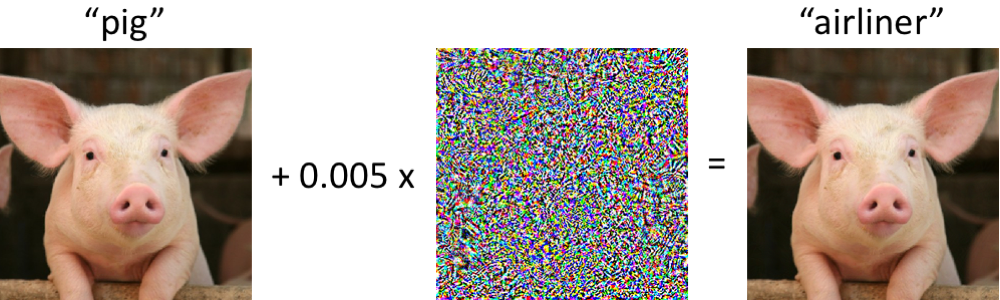
\includegraphics[scale=0.4]{figures/piggie.png}
  \caption{Hyökkäys lentoyhtiötä kohtaan. \citep{adversexamples}}
\end{figure}